\textbf{Les angles marqués sont-ils alternes-internes, correspondants ou ni l'un, ni l'autre ?}
\begin{multicols}{3}
\begin{enumerate}
	\item \begin{minipage}[t]{\linewidth} 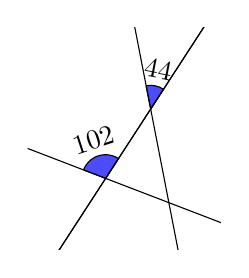
\begin{tikzpicture}[baseline,scale = 0.3]

    \tikzset{
      point/.style={
        thick,
        draw,
        cross out,
        inner sep=0pt,
        minimum width=5pt,
        minimum height=5pt,
      },
    }
    \clip (-4.390019349521659,-4.69335283972712) rectangle (3.78572476438357,4.702887402261128);
    	\draw  [color={black},preaction={fill,color = {blue},opacity = 0.7}] (0.626149557145996,2.2396330353657996) -- (0.8169585525225405,1.2580058519181354) -- (1.3615975875375679,2.0966764198635595) arc (56.72:100.72:1) ;
	\draw[color={black}] (-8.723491216304707,50.33936502430133)--(10.548217316726333,-48.804980503912724);
	\draw[color={black}] (-26.414993198228814,-40.67552254535305)--(28.59354933828892,44.030204817134745);
	\draw  [color={black},preaction={fill,color = {blue},opacity = 0.7}] (-2.0228584965272556,-1.3189731863455467) -- (-1.0892780700300544,-1.6773411358908479) -- (-0.5446390350150268,-0.8386705679454244) arc (56.72:158.72:1) ;
	\draw[color={black}] (-47.76829939489014,16.241056341374165)--(46.523323681327234,-19.954106562701163);
	\draw[color={black}] (-28.321229820781415,-43.610869533162045)--(26.687312715736333,41.094857829325775);
	\draw [color={black}] (1.14,2.93) node[anchor = center,scale=1, rotate = -10.995039999999989] {\ang{44}};
	\draw [color={black}] (-1.61,-0.06) node[anchor = center,scale=1, rotate = -341.99936] {\ang{102}};

\end{tikzpicture}\\ \end{minipage}
	\item \begin{minipage}[t]{\linewidth} 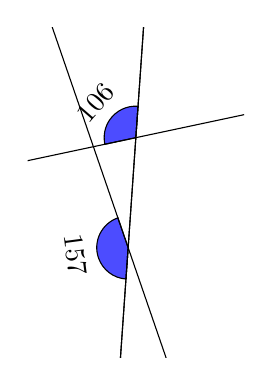
\begin{tikzpicture}[baseline,scale = 0.4]

    \tikzset{
      point/.style={
        thick,
        draw,
        cross out,
        inner sep=0pt,
        minimum width=5pt,
        minimum height=5pt,
      },
    }
    \clip (-3.329808091585229,-5.487820251299121) rectangle (3.539077512817605,4.989038226169209);
    	\draw  [color={black},preaction={fill,color = {blue},opacity = 0.7}] (-0.8735128901176171,1.2884343845719772) -- (0.1046347106161884,1.4963460753897364) -- (0.17439118436031364,2.4939101256495606) arc (85.69:191.69:1) ;
	\draw[color={black}] (-48.802745326074096,-8.899238465498234)--(49.99016234804028,12.099842307095466);
	\draw[color={black}] (-3.3831889765900853,-48.381856437601485)--(3.662214871566587,52.372112638640786);
	\draw  [color={black},preaction={fill,color = {blue},opacity = 0.7}] (-0.20926942123237727,-2.992692150779473) -- (-0.1395129474882513,-1.9951281005196484) -- (-0.4650811019454078,-1.0496095249203314) arc (109.17:266.17:1) ;
	\draw[color={black}] (-16.41792067034609,45.280800679446195)--(16.464462929826745,-50.21657545608481);
	\draw[color={black}] (-3.627336634694524,-51.87333061351086)--(3.4180672134621473,48.88063846273138);
	\draw [color={black}] (-1.18,2.61) node[anchor = center,scale=1, rotate = -311.0002] {\ang{106}};
	\draw [color={black}] (-1.82,-2.22) node[anchor = center,scale=1, rotate = -82.50011] {\ang{157}};

\end{tikzpicture}\\ \end{minipage}
	\item \begin{minipage}[t]{\linewidth} 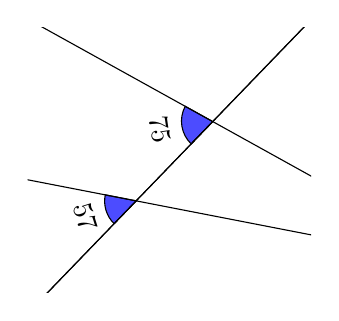
\begin{tikzpicture}[baseline,scale = 0.4]

    \tikzset{
      point/.style={
        thick,
        draw,
        cross out,
        inner sep=0pt,
        minimum width=5pt,
        minimum height=5pt,
      },
    }
    \clip (-4.486869106031488,-4.000328516779962) rectangle (4.5131758623361815,4.4200065683925605);
    	\draw  [color={black},preaction={fill,color = {blue},opacity = 0.7}] (0.6946583704589984,0.7193398003386509) -- (1.3893167409179954,1.4386796006773026) -- (0.5146970337785991,1.9234892209236392) arc (151.86:226.86:1) ;
	\draw[color={black}] (-42.34166861605179,25.679160612994153)--(45.99492180502718,-23.286611031885883);
	\draw[color={black}] (-33.343601782031854,-34.52831041625525)--(36.816893634326846,38.12500941794851);
	\draw  [color={black},preaction={fill,color = {blue},opacity = 0.7}] (-1.7366459261474938,-1.798349500846627) -- (-1.0419875556884963,-1.0790097005079757) -- (-2.0236147391361605,-0.8882007051314311) arc (168.54:225.54:1) ;
	\draw[color={black}] (-50.123346728071695,8.461440068319265)--(49.02099880014237,-10.810268464711761);
	\draw[color={black}] (-35.77490607863836,-37.04599971744053)--(34.38558933772037,35.60732011676323);
	\draw [color={black}] (-0.29,1.19) node[anchor = center,scale=1, rotate = -81.50019] {\ang{75}};
	\draw [color={black}] (-2.66,-1.59) node[anchor = center,scale=1, rotate = -72.49962] {\ang{57}};

\end{tikzpicture}\\ \end{minipage}
	\item \begin{minipage}[t]{\linewidth} 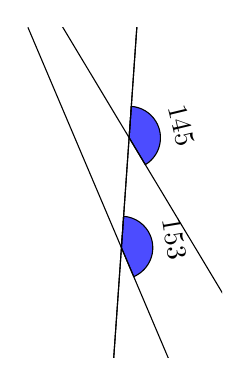
\begin{tikzpicture}[baseline,scale = 0.4]

    \tikzset{
      point/.style={
        thick,
        draw,
        cross out,
        inner sep=0pt,
        minimum width=5pt,
        minimum height=5pt,
      },
    }
    \clip (-3.081320233229482,-4.989038226169209) rectangle (3.0925418121643005,5.487820251299121);
    	\draw  [color={black},preaction={fill,color = {blue},opacity = 0.7}] (0.20926942123237668,2.992692150779472) -- (0.1395129474882511,1.9951281005196482) -- (0.6545510223983052,1.1379607998175363) arc (-58.68:86.32:1) ;
	\draw[color={black}] (-25.612390798014463,44.85349313562526)--(26.406454767901018,-41.72040423528807);
	\draw[color={black}] (-3.348310739718021,-47.88307441247155)--(3.6970931084386485,52.87089466377067);
	\draw  [color={black},preaction={fill,color = {blue},opacity = 0.7}] (-0.034878236872062596,-0.4987820251299113) -- (-0.10463471061618815,-1.496346075389736) -- (0.2860964178730856,-2.4168509288421767) arc (-66.73:86.27:1) ;
	\draw[color={black}] (-19.641191135079886,44.52889659723229)--(19.822652842336783,-48.44209360146421);
	\draw[color={black}] (-3.5924583978224613,-51.37454858838095)--(3.45294545033421,49.379420487861296);
	\draw [color={black}] (1.79,2.39) node[anchor = center,scale=1, rotate = -76.50006] {\ang{145}};
	\draw [color={black}] (1.57,-1.22) node[anchor = center,scale=1, rotate = -80.50002] {\ang{153}};

\end{tikzpicture}\\ \end{minipage}
	\item \begin{minipage}[t]{\linewidth} 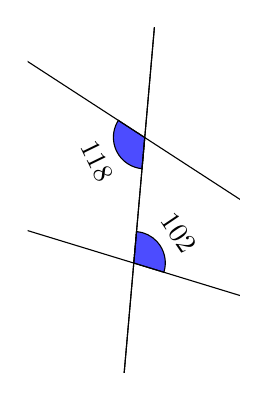
\begin{tikzpicture}[baseline,scale = 0.4]

    \tikzset{
      point/.style={
        thick,
        draw,
        cross out,
        inner sep=0pt,
        minimum width=5pt,
        minimum height=5pt,
      },
    }
    \clip (-3.543225753384422,-5.480973490458728) rectangle (3.1946027823937895,5.480973490458728);
    	\draw  [color={black},preaction={fill,color = {blue},opacity = 0.7}] (0.08715574274765758,0.9961946980917454) -- (0.17431148549531622,1.9923893961834909) -- (-0.6643590824501077,2.537028431198518) arc (147.48:265.48:1) ;
	\draw[color={black}] (-41.75921691177589,29.22434114693484)--(42.94651045071194,-25.784201389582886);
	\draw[color={black}] (-4.183475651887591,-47.8173455084038)--(4.619254365625881,52.79831899886253);
	\draw  [color={black},preaction={fill,color = {blue},opacity = 0.7}] (-0.08715574274765814,-0.9961946980917457) -- (-0.17431148549531658,-1.992389396183491) -- (0.7819932704677189,-2.284761100906228) arc (-17.25:84.75:1) ;
	\draw[color={black}] (-47.98954928364709,12.626195839953347)--(48.597231068619486,-16.903346337043065);
	\draw[color={black}] (-4.532098622878223,-51.80212430077077)--(4.270631394635249,48.81354020649553);
	\draw [color={black}] (-1.35,1.25) node[anchor = center,scale=1, rotate = -64.00014] {\ang{118}};
	\draw [color={black}] (1.24,-1.04) node[anchor = center,scale=1, rotate = -55.999719999999996] {\ang{102}};

\end{tikzpicture}\\ \end{minipage}
	\item \begin{minipage}[t]{\linewidth} 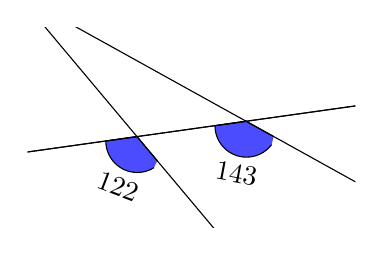
\begin{tikzpicture}[baseline,scale = 0.4]

    \tikzset{
      point/.style={
        thick,
        draw,
        cross out,
        inner sep=0pt,
        minimum width=5pt,
        minimum height=5pt,
      },
    }
    \clip (-4.956206309337067,-3.0958463764853414) rectangle (5.451340343707852,3.249879544778853);
    	\draw  [color={black},preaction={fill,color = {blue},opacity = 0.7}] (2.8551558446225362,-0.20646341832620585) -- (1.9805361374831405,0.27834620192013104) -- (0.9902680687415701,0.13917310096006552) arc (-180:-37:1) ;
	\draw[color={black}] (-41.75044921948663,24.518827214236982)--(46.58614120159231,-24.446944430643057);
	\draw[color={black}] (-47.53286729959539,-6.680308846083142)--(52.48420764330324,7.37617435088347);
	\draw  [color={black},preaction={fill,color = {blue},opacity = 0.7}] (-0.842614493425816,-0.9748040945590766) -- (-1.4854021031123552,-0.20875965144009823) -- (-2.475670171853926,-0.34793275240016364) arc (-180:-58:1) ;
	\draw[color={black}] (-33.62478258743933,38.09346250450881)--(31.296765990901154,-39.27702625050798);
	\draw[color={black}] (-50.99880554019087,-7.16741469944337)--(49.01826940270773,6.889068497523239);
	\draw [color={black}] (1.67,-1.39) node[anchor = center,scale=1, rotate = -10.49892] {\ang{143}};
	\draw [color={black}] (-2.09,-1.8) node[anchor = center,scale=1, rotate = -20.99966] {\ang{122}};

\end{tikzpicture}\\ \end{minipage}
	\item \begin{minipage}[t]{\linewidth} 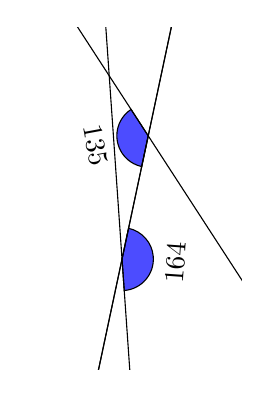
\begin{tikzpicture}[baseline,scale = 0.4]

    \tikzset{
      point/.style={
        thick,
        draw,
        cross out,
        inner sep=0pt,
        minimum width=5pt,
        minimum height=5pt,
      },
    }
    \clip (-3.4116822670772207,-5.448987352247084) rectangle (3.387356724494242,5.390738003669028);
    	\draw  [color={black},preaction={fill,color = {blue},opacity = 0.7}] (0.20791169081775973,0.9781476007338062) -- (0.4158233816355189,1.9562952014676114) -- (-0.12881565337950807,2.794965769413035) arc (123.28:258.28:1) ;
	\draw[color={black}] (-26.816128369115834,43.8898235987388)--(28.1924141674019,-40.815903763749);
	\draw[color={black}] (-9.979761159252451,-46.95108483522266)--(11.01931961334125,51.84182283889169);
	\draw  [color={black},preaction={fill,color = {blue},opacity = 0.7}] (-0.20791169081775984,-0.9781476007338058) -- (-0.4158233816355195,-1.9562952014676112) -- (-0.3460669078913941,-2.9538592517274354) arc (-85.69:78.31:1) ;
	\draw[color={black}] (-3.903647068841793,47.9219073115236)--(3.1417567793148793,-52.832061764718645);
	\draw[color={black}] (-10.811407922523491,-50.86367523815789)--(10.187672850070213,47.92923243595647);
	\draw [color={black}] (-1.26,1.65) node[anchor = center,scale=1, rotate = -79.4997] {\ang{135}};
	\draw [color={black}] (1.28,-2.07) node[anchor = center,scale=1, rotate = 85.99994] {\ang{164}};

\end{tikzpicture}\\ \end{minipage}
	\item \begin{minipage}[t]{\linewidth} 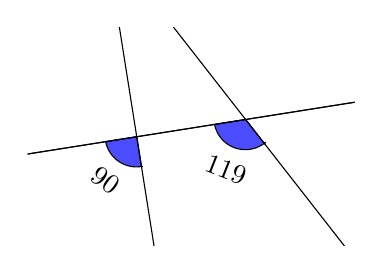
\begin{tikzpicture}[baseline,scale = 0.4]

    \tikzset{
      point/.style={
        thick,
        draw,
        cross out,
        inner sep=0pt,
        minimum width=5pt,
        minimum height=5pt,
      },
    }
    \clip (-4.94459753267812,-3.6977167193457596) rectangle (5.438441702975689,3.228413324225068);
    	\draw  [color={black},preaction={fill,color = {blue},opacity = 0.7}] (2.5910381565159337,-0.4751418235262608) -- (1.9753766811902758,0.3128689300804615) -- (0.9876883405951378,0.15643446504023095) arc (-168.54:-49.53999999999999:1) ;
	\draw[color={black}] (-28.807697085092634,39.71340661041656)--(33.374111922798846,-39.87567950386236);
	\draw[color={black}] (-47.40904034856661,-7.508854321931083)--(52.3474820515423,8.291026647132238);
	\draw  [color={black},preaction={fill,color = {blue},opacity = 0.7}] (-1.3250980458524761,-1.2223400381554839) -- (-1.4815325108927069,-0.234651697560346) -- (-2.4692208514878446,-0.3910861626005768) arc (-168.54:-78.53999999999999:1) ;
	\draw[color={black}] (-9.303255762904255,49.149765332196544)--(6.496625206159072,-50.606757067912376);
	\draw[color={black}] (-50.865949540649595,-8.05637494957189)--(48.89057285945932,7.743506019491428);
	\draw [color={black}] (1.35,-1.27) node[anchor = center,scale=1, rotate = -21.49967] {\ang{119}};
	\draw [color={black}] (-2.48,-1.61) node[anchor = center,scale=1, rotate = -36.00042] {\ang{90}};

\end{tikzpicture}\\ \end{minipage}
	\item \begin{minipage}[t]{\linewidth} 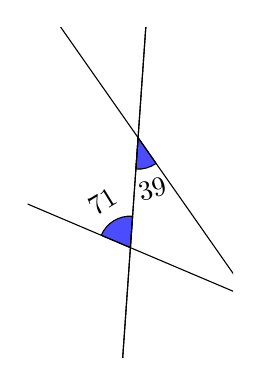
\begin{tikzpicture}[baseline,scale = 0.4]

    \tikzset{
      point/.style={
        thick,
        draw,
        cross out,
        inner sep=0pt,
        minimum width=5pt,
        minimum height=5pt,
      },
    }
    \clip (-3.3661492709735095,-4.989038226169209) rectangle (3.1568798497411326,5.487820251299121);
    	\draw  [color={black},preaction={fill,color = {blue},opacity = 0.7}] (0.7130893838392963,1.1759760562306565) -- (0.1395129474882508,1.9951281005196482) -- (0.06975647374412534,0.9975640502598244) arc (-93.77:-54.769999999999996:1) ;
	\draw[color={black}] (-28.539308870064048,42.95273031496924)--(29.391911201391594,-39.78162615821893);
	\draw[color={black}] (-3.348310739718021,-47.88307441247155)--(3.6970931084386485,52.87089466377067);
	\draw  [color={black},preaction={fill,color = {blue},opacity = 0.7}] (-1.0251395640686283,-1.1056149469004621) -- (-0.10463471061618831,-1.496346075389736) -- (-0.034878236872062915,-0.498782025129912) arc (85.69:156.69:1) ;
	\draw[color={black}] (-46.12987738323821,18.040210349073945)--(46.841112815458274,-21.42363362834269);
	\draw[color={black}] (-3.5924583978224613,-51.37454858838095)--(3.45294545033421,49.379420487861296);
	\draw [color={black}] (0.59,0.36) node[anchor = center,scale=1, rotate = 15.49952] {\ang{39}};
	\draw [color={black}] (-0.99,-0.05) node[anchor = center,scale=1, rotate = -328.49966] {\ang{71}};

\end{tikzpicture}\\ \end{minipage}
\end{enumerate}
\end{multicols}
